\documentclass{beamer}

\mode<presentation>
{
\usetheme[width=0.7in]{Hannover}
}

\usepackage[english]{babel}
\usepackage{amsthm}
\usepackage{amssymb}
\usepackage{comment} % to let us comment stuff out

\usepackage{times}
\usepackage{physics}
\usepackage{yquant}
\useyquantlanguage{groups}

\usepackage{subcaption}
\usepackage{tikz}
\usetikzlibrary{quantikz,fit,quotes,svg.path}
\newcommand{\h}[1]{\mintinline{haskell}{#1}}

\newcommand{\x}{\textsc{x}}
\newcommand{\cx}{\textsc{cx}}
\newcommand{\ccx}{\textsc{ccx}}
\newcommand{\cccx}{\textsc{cccx}}
\newcommand{\qket}[1]{\ket{\tilde{#1}}}
\newcommand{\preim}[2]{\{\cdot\stackrel{#1}{\longleftarrow}{#2}\}}
\newcommand{\finset}[1]{[\mathbf{#1}]}
\newcommand{\red}[1]{{\color{red}{#1}}}
\newcommand{\Bool}{\ensuremath{\mathbb{B}}}

% \usepackage{multirow}
% \usepackage{totpages}
\usepackage{hyperref}
% \usepackage{booktabs}

\hypersetup{
  urlcolor=blue,
  linkcolor=blue,
  colorlinks=true
}

\newtheorem{defn}{Definition}
\newtheorem{prob}{Problem}

\usepackage{listings}
\lstset{columns=flexible,
        language=haskell}
%\usepackage{tikz}
%\usetikzlibrary{positioning}

\newcommand{\blt}{- } %used for bullets in a list

\newcounter{datadefnum} %Datadefinition Number
\newcommand{\ddthedatadefnum}{DD\thedatadefnum}
\newcommand{\ddref}[1]{DD\ref{#1}}

\newcommand{\colAwidth}{0.1\textwidth}
\newcommand{\colBwidth}{0.8\textwidth}

\renewcommand{\arraystretch}{1.1} %so that tables with equations do not look 
%crowded

\pgfdeclareimage[height=0.7cm]{logo}{../WG211/McMasterLogo}
\title[\pgfuseimage{logo}] % (optional, use only with long paper titles)
{Symbolic Evaluation of Hadamard-Toffoli Quantum Circuits}

\author[]{\underline{Jacques Carette}, Amr Sabry, Gerardo Ortiz}

%\date[Aug 18, 2022] % (optional, should be abbreviation of conference name)
%{WG 2.11, Odense, Denmark}

\pgfdeclareimage[height=0.5cm]{Mac-logo}{McMasterLogo}
\logo{\pgfuseimage{Mac-logo}}

% If you wish to uncover everything in a step-wise fashion, uncomment
% the following command: 

%\beamerdefaultoverlayspecification{<+->}

\beamertemplatenavigationsymbolsempty 

\usepackage{color}

%% Useful abbreviations

\newcommand{\half}{\frac{1}{2}}
\newcommand{\shalf}{\frac{1}{\sqrt{2}}}

\newcommand{\pub}[1]{\textcolor{purple}{#1}}
\newcommand{\blu}[1]{\textcolor{blue}{#1}}

\begin{document}


%%%%%%%%%%%%%%%%%%%%%%%%%%%%%%%%%%%%%%
\hoffset=-.4in %removing side bar for these frames
\begin{frame}[plain]

\titlepage

\end{frame}
\hoffset=0in %restore

%%%%%%%%%%%%%%%%%%%%%%%%%%%%%%%%%%%%%%

\section[Introduction]{Introduction}

% not sure if 3 slides or just 1 with transitions?
\subsection[Reversible]{Reversible Gates}

\begin{frame}
  \frametitle{Reversible gates}

\begin{minipage}{0.48\textwidth}
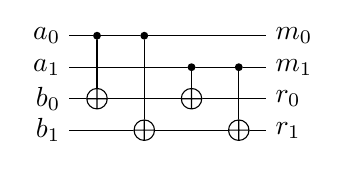
\begin{tikzpicture}[scale=1.0,every label/.style={rotate=40, anchor=south west}]
\begin{yquant*}[operators/every barrier/.append style={red, thick}]
    qubit {$a_0$} a0;
    qubit {$a_1$} a1;
    qubit {$b_0$} b0;
    qubit {$b_1$} b1;
    cnot b0 | a0;
    cnot b1 | a0;
    cnot b0 | a1;
    cnot b1 | a1;
    align -;
    output {$m_0$} a0;
    output {$m_1$} a1;
    output {$r_0$} b0;
    output {$r_1$} b1;
\end{yquant*}
\end{tikzpicture}
\end{minipage}
\begin{minipage}{0.48\textwidth}
\[\begin{array}{rcl}
\cx(0,b) &=& (0,b) \\
\cx(1,b) &=& (1,\overline{b})
\end{array}\]
\end{minipage}

\vspace*{6mm}
So, writing inputs/outputs horizontally:

\vspace*{3mm}
$ \begin{array}{rcl}
\ket{0111} & \Rightarrow & \ket{0111} \\
           & \Rightarrow & \ket{0111} \\
           & \Rightarrow & \ket{0101} \\
           & \Rightarrow & \ket{0100}
\end{array}
$
\qquad\qquad
$ \begin{array}{rcl}
\ket{1010} & \Rightarrow & \ket{1000} \\
           & \Rightarrow & \ket{1001} \\
           & \Rightarrow & \ket{1001}  \\
           & \Rightarrow & \ket{1001} \\
\end{array}
$

\vspace*{3mm}
$ \begin{array}{rcl}
\ket{1100} & \Rightarrow & \ket{1110} \\
           & \Rightarrow & \ket{1111} \\
           & \Rightarrow & \ket{1101} \\
           & \Rightarrow & \ket{1100}  \\
\end{array}
$
\qquad\qquad
$ \begin{array}{rcl}
\ket{1111} & \Rightarrow & \ket{1101}\\
           & \Rightarrow & \ket{1100} \\
           & \Rightarrow & \ket{1110} \\
           & \Rightarrow & \ket{1111} \\
\end{array}
$
\end{frame}

%%%%%%%%%%%%%%%%%%%%%%%%%%%%%%%%%%%%%%

\subsection[Superposition]{Superpositions}

\begin{frame}
  \frametitle{Superpositions}
  
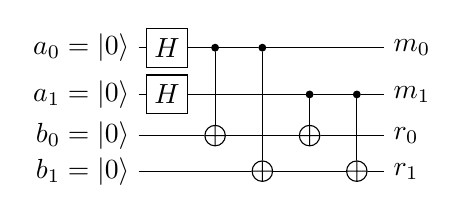
\begin{tikzpicture}[scale=1.0,every label/.style={rotate=40, anchor=south west}]
\begin{yquant*}[operators/every barrier/.append style={red, thick}]
    qubit {$a_0=\ket0$} a0;
    qubit {$a_1=\ket0$} a1;
    qubit {$b_0=\ket0$} b0;
    qubit {$b_1=\ket0$} b1;
    box {$H$} a0;
    box {$H$} a1;
    cnot b0 | a0;
    cnot b1 | a0;
    cnot b0 | a1;
    cnot b1 | a1;
    align -;
    output {$m_0$} a0;
    output {$m_1$} a1;
    output {$r_0$} b0;
    output {$r_1$} b1;
\end{yquant*}
\end{tikzpicture}
\[\begin{array}{rclcl}
H\ket{0} &=& \shalf\ket{0} + \shalf\ket{1}
         &=& \frac{1}{\sqrt{2}} (\ket{0} + \ket{1})
 \end{array}\]

\begin{overprint}
\onslide<1>
So the top two wires are in the state
\[ \shalf(\ket{0}+\ket{1}) \otimes 
   \shalf(\ket{0}+\ket{1}) 
   = 
\half(\ket{00} + \ket{10} + \ket{01} + \ket{11})
\]
\onslide<2>
Thus for the whole circuit:
\[\begin{array}{rcl}
    \ket{0000} &\Rightarrow&
      \half (\ket{0000} + \ket{0100} + \ket{1000} + \ket{1100}) \\
    &\Rightarrow& 
      \half (\ket{0000} + \ket{0100} + \ket{1010} + \ket{1110}) \\
    &\Rightarrow& 
      \half (\ket{0000} + \ket{0100} + \ket{1011} + \ket{1111}) \\
    &\Rightarrow& 
      \half (\ket{0000} + \ket{0110} + \ket{1011} + \ket{1101}) \\
    &\Rightarrow& 
      \half (\ket{0000} + \ket{0111} + \ket{1011} + \ket{1100}) 
 \end{array}\]
\end{overprint}
\end{frame}

\subsection[Symbolic]{Qubits as symbolic variables}

\begin{frame}
  \frametitle{Symbolic Execution (\pub{new})}
  
Replace $\shalf (\ket{0} + \ket{1})$ by a symbolic variable:

\begin{center}
\begin{yquantgroup}
\registers{
  qubit {} a0;
  qubit {} a1;
  qubit {$\ket0$} b0;
  qubit {$\ket0$} b1;
}
\circuit{
    init {$\ket0$} a0; 
    init {$\ket0$} a1; 
    box {$H$} a0;
    box {$H$} a1;
    cnot b0 | a0;
    cnot b1 | a0;
    cnot b0 | a1;
    cnot b1 | a1;
}
\equals[$\rightsquigarrow$]
\circuit{
    init {$x$} a0; 
    init {$y$} a1;
    cnot b0 | a0;
    cnot b1 | a0;
    cnot b0 | a1;
    cnot b1 | a1;
 } 
\end{yquantgroup}
\end{center}

Maintain formula in algebraic normal form (ANF).

So
\[\begin{array}{rcl}
    \ket{xy00} &\Rightarrow&
      \ket{xyx0} \\
    &\Rightarrow& 
      \ket{xyxx} \\
    &\Rightarrow& 
      \ket{xy(x\oplus y)x} \\
    &\Rightarrow& 
      \ket{xy(x\oplus y)(x\oplus y)} 
 \end{array}\]
\end{frame}

%%%%%%%%%%%%%%%%%%%%%%%%%%%%%%%%%%%%%%%%%%%%%%%%%%%%%%%%%%%%%%%
\section[Big Picture]{Big Picture}

\subsection[Retrodictive]{Template and Retrodictive}
\begin{frame}
  \frametitle{Quantum Circuits}
\begin{overprint}
\onslide<1>
    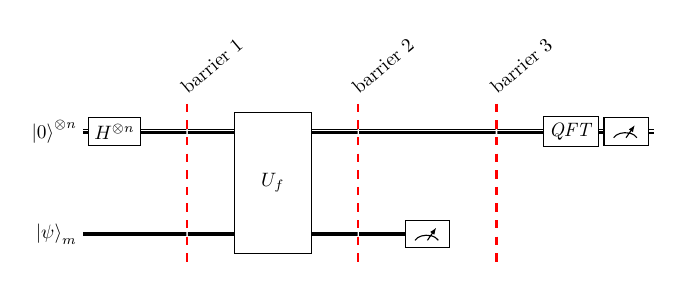
\begin{tikzpicture}[scale=0.7,every label/.style={rotate=40, anchor=south west}]
    \begin{yquant*}[operators/every barrier/.append style={red, thick},
        operator/minimum width=7mm,
        operator/separation=1mm,
        register/separation=10mm]
    qubits {$\ket0^{\otimes n}$} a;
    qubits {$\ket{\psi}_m$} b;
    box {$H^{\otimes n}$} a;
    ["barrier 1"]
    barrier (-);
    [x radius=7mm, y radius=7mm]
    box {$U_f$} (a,b);
    ["barrier 2"]
    barrier (-);
    measure b;
    discard b;
    ["barrier 3"]
    barrier (-);
    box {$\mathit{QFT}$} a;
    measure a;
    \end{yquant*}
  \end{tikzpicture}

\onslide<2>
  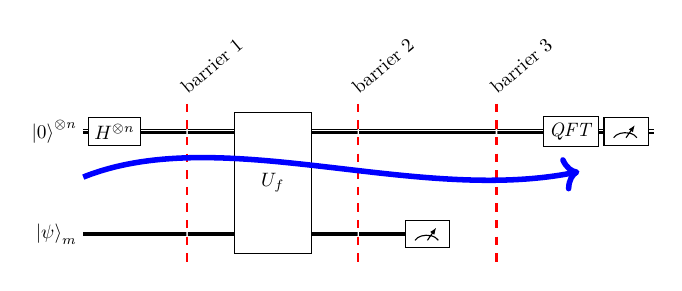
\begin{tikzpicture}[scale=0.7,every label/.style={rotate=40, anchor=south west}]
    \begin{yquant*}[operators/every barrier/.append style={red, thick},
        operator/minimum width=7mm,
        operator/separation=1mm,
        register/separation=10mm]
    qubits {$\ket0^{\otimes n}$} a;
    qubits {$\ket{\psi}_m$} b;
    box {$H^{\otimes n}$} a;
    ["barrier 1"]
    barrier (-);
    [x radius=7mm, y radius=7mm]
    box {$U_f$} (a,b);
    ["barrier 2"]
    barrier (-);
    measure b;
    discard b;
    ["barrier 3"]
    barrier (-);
    box {$\mathit{QFT}$} a;
    measure a;
    \end{yquant*}
    \draw[line width=2pt, ->, blue] (0,-1.1) .. controls (2.5,-0.1) and (6,-1.6) .. (9,-1);
  \end{tikzpicture}

\onslide<3>
  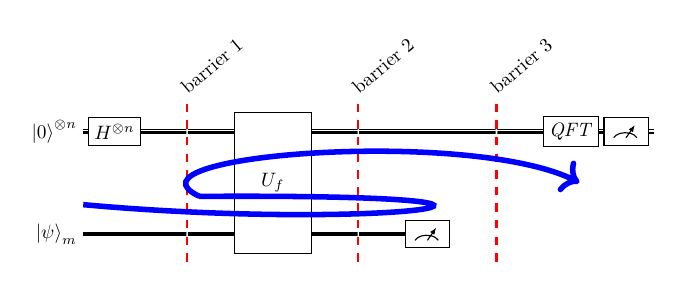
\begin{tikzpicture}[scale=0.7,every label/.style={rotate=40, anchor=south west}]
    \begin{yquant*}[operators/every barrier/.append style={red, thick},
        operator/minimum width=7mm,
        operator/separation=1mm,
        register/separation=10mm]
    qubits {$\ket0^{\otimes n}$} a;
    qubits {$\ket{\psi}_m$} b;
    box {$H^{\otimes n}$} a;
    ["barrier 1"]
    barrier (-);
    [x radius=7mm, y radius=7mm]
    box {$U_f$} (a,b);
    ["barrier 2"]
    barrier (-);
    measure b;
    discard b;
    ["barrier 3"]
    barrier (-);
    box {$\mathit{QFT}$} a;
    measure a;
  \end{yquant*}
  \draw[line width=2pt, blue] (0,-1.6) .. controls (5.5,-2.1) and (10,-1.4) .. (2.1,-1.45);
  \draw[line width=2pt, ->, blue] (2.11,-1.45) .. controls (0.5,-0.7) and (7,-0.2) .. (9,-1.2);
  \end{tikzpicture}

\end{overprint}
\begin{itemize}
\item $U_f$ is a \emph{classical reversible} circuit representing the
  function of interest; 
\item $H$ is the Hadamard gate; it is used to introduce \emph{quantum
    parallelism} to evaluate $U_f$ for many inputs simultaneously.
\item $\mathit{QFT}$ is the Quantum Fourier Transform used to analyze
  the spectral properties of the output.  
\end{itemize}
\end{frame}

\subsection[Cost Models]{Cost Models}

\begin{frame}
  \frametitle{Cost Models}
  \begin{itemize}
\item White-box model: \emph{We} implement $U_f$ and the cost of
  implementing it and the cost of using it is counted as part of the
  overall complexity
\item Black-box model: ``Someone'' implements $U_f$ and gives us
  access to it; the complexity analysis only counts the number of
  times $U_f$ is used. There are different cases based on what kind of
  access we are given:
  \begin{itemize}
    \item Query $U_f$ on a classical input 
    \item Query $U_f$ on a quantum superposition
    \item Query $U_f$ on a \emph{symbolic formula} (\textbf{NEW!})
  \end{itemize}
    \end{itemize}
  
\end{frame}

%%%%%%%%%%%%%%%%%%%%%%%%%%%%%%%%%%%%%%%%%%%%%%%%%%%%%%%%%%%%%%%

\section[Examples]{Examples}
% - Examples of quantum algorithms (how much detail?)

%%%%%%%%%%%%%%%%%%%%%%%%%%%%%%%%%%%%%%

\begin{frame}

\frametitle{Examples}

\begin{enumerate}
  \item Deutsch
  \item Deutsch-Jozsa
  \item Bernstein-Varizani
  \item Simon
  \item Grover
  \item Shor
\end{enumerate}

\end{frame}

%%%%%%%%%%%%%%%%%%%%%%%%%%%%%%%%%%%%%%

\section[Software]{Software Description}
\subsection[Requirements]{Requirements}
\begin{frame}
  \frametitle{Requirements}
  Variabilities:
\begin{enumerate}
  \item \pub{multiple representations} of boolean \blu{values},
  \item \pub{multiple representations} of boolean \blu{formulae}, 
  \item \pub{different evaluation} means (directly, symbolically, forwards,
    backwards, retrodictive).
\end{enumerate}

\noindent Possible to implement:
\begin{enumerate}
    \setcounter{enumi}{3}
  \item a \pub{reusable representation} of our circuits,
  \item a \pub{reusable representation} of the inputs, outputs and ancillae,
  \item a \pub{synthesis algorithm} for $\Bool^n\rightarrow\Bool$ functions
  \item a \pub{reusable library} of circuits
\end{enumerate}

Also, non-functional characteristics to hold:
\begin{enumerate}
    \setcounter{enumi}{7}
  \item evaluation of \blu{reasonably-sized circuits} should be 
    \pub{relatively efficient}.
\end{enumerate}

\end{frame}

\subsection[Design]{Design}

%%%%%%%%%%%%%%%%%%%%%%%%%%%%%%%%%%%%%%

\section[Evaluation]{Evaluation}
\subsection[Running]{Running examples}
\subsection[Timings]{Timings}
\subsection[Complexity]{Complexity}

\begin{frame}

\frametitle{Deutsch}

  \begin{prob}
Given $f : \Bool\rightarrow\Bool$, decide if $f$ is 
\emph{constant} or \emph{balanced}.
  \end{prob}

\pause

\begin{defn}
  A boolean function is \textbf{balanced} if it outputs the same number of
  0/1 outputs.
\end{defn}

\pause

\vspace*{1cm}
$\ket{x}\ket{y} \rightarrow\ket{x}\ket{f(x)\oplus y}$
\end{frame}


%%%%%%%%%%%%%%%%%%%%%%%%%%%%%%%%%%%%%%

\begin{frame}

\frametitle{Deutsch-Josza}

  \begin{prob}Given $f : \Bool^n\rightarrow\Bool$, where $f$ is known to be
\emph{constant} or \emph{balanced}, decide which one it is.
  \end{prob}

\pause

Sample outputs:
\begin{itemize}
\item $0 = 0$
\item $x_0 = 0$,
\item $x_0 \oplus x_1 \oplus x_2 \oplus x_3 \oplus
    x_4 \oplus x_5 = 0$, and
\item $1 \oplus x_3x_5 \oplus x_2x_4 \oplus x_1x_5
\oplus x_0x_3 \oplus x_0x_2 \oplus x_3x_4x_5 \oplus x_2x_3x_5 \oplus
x_1x_3x_5 \oplus x_0x_3x_5 \oplus x_0x_1x_4 \oplus x_0x_1x_2 \oplus
x_2x_3x_4x_5 \oplus x_1x_3x_4x_5 \oplus x_1x_2x_4x_5 \oplus
x_1x_2x_3x_5 \oplus x_0x_3x_4x_5 \oplus x_0x_2x_4x_5 \oplus
x_0x_2x_3x_5 \oplus x_0x_1x_4x_5 \oplus x_0x_1x_3x_5 \oplus
x_0x_1x_3x_4 \oplus x_0x_1x_2x_4 \oplus x_0x_1x_2x_4x_5 \oplus
x_0x_1x_2x_3x_5 \oplus x_0x_1x_2x_3x_4 = 0$.
\end{itemize}

  But how to \emph{decide}? Easy: if it mentions a variable, it's balanced.
\end{frame}

%%%%%%%%%%%%%%%%%%%%%%%%%%%%%%%%%%%%%%

\begin{frame}

\frametitle{Bernstein-Varizani, Simon}

Bernstein-Varizani
\begin{prob}
    Given $f : \Bool^n\rightarrow\Bool$, where $f$ is known to be
of the shape $\sum_i s_i x_i \mod 2$ for some $s\in\Bool^n$ and $s_i$ is its
bit decomposition. Find $s$.
\end{prob}

\pause

Simon
\begin{prob}
    Given $f : \Bool^n\rightarrow\Bool$, where it is known that
    there exist $a$ such that $\forall x. f(x) = f(x + a)$. Find $a$.
\end{prob}

\end{frame}

%%%%%%%%%%%%%%%%%%%%%%%%%%%%%%%%%%%%%%

\begin{frame}

  \frametitle{Grover}

\begin{prob}
    Given $f : \Bool^n\rightarrow\Bool$ where there exists a unique $x$
    such that $f(x)=1$. Find $x$.
\end{prob}

\pause

$n=4$, $w$ in the range $\{0..15\}$
  {\tiny
\begin{tabular}{ll}
$u=0$ & 
  $\red{1} \oplus x_3 \oplus x_2 \oplus x_1 \oplus x_0 \oplus x_2x_3 \oplus x_1x_3 \oplus x_1x_2 \oplus x_0x_3 \oplus x_0x_2 \oplus x_0x_1 \oplus x_1x_2x_3 \oplus x_0x_2x_3$ \\
   &\quad $\oplus ~x_0x_1x_3 \oplus x_0x_1x_2 \oplus x_0x_1x_2x_3$ \\
$u=1$ & 
  $\red{x_0} \oplus x_0x_3 \oplus x_0x_2 \oplus x_0x_1 \oplus x_0x_2x_3 \oplus x_0x_1x_3 \oplus x_0x_1x_2 \oplus x_0x_1x_2x_3$ \\
$u=2$ &
  $\red{x_1} \oplus x_1x_3 \oplus x_1x_2 \oplus x_0x_1 \oplus x_1x_2x_3 \oplus x_0x_1x_3 \oplus x_0x_1x_2 \oplus x_0x_1x_2x_3$ \\
$u=3$ &
  $\red{x_0x_1} \oplus x_0x_1x_3 \oplus x_0x_1x_2 \oplus x_0x_1x_2x_3$ \\
$u=4$ &
  $\red{x_2} \oplus x_2x_3 \oplus x_1x_2 \oplus x_0x_2 \oplus x_1x_2x_3 \oplus x_0x_2x_3 \oplus x_0x_1x_2 \oplus x_0x_1x_2x_3$ \\
$u=5$ &
  $\red{x_0x_2} \oplus x_0x_2x_3 \oplus x_0x_1x_2 \oplus x_0x_1x_2x_3$ \\
$u=6$ &
  $\red{x_1x_2} \oplus x_1x_2x_3 \oplus x_0x_1x_2 \oplus x_0x_1x_2x_3$ \\
$u=7$ &
  $\red{x_0x_1x_2} \oplus x_0x_1x_2x_3$ \\
$u=8$ &
  $\red{x_3} \oplus x_2x_3 \oplus x_1x_3 \oplus x_0x_3 \oplus x_1x_2x_3 \oplus x_0x_2x_3 \oplus x_0x_1x_3 \oplus x_0x_1x_2x_3$ \\
$u=9$ &
  $\red{x_0x_3} \oplus x_0x_2x_3 \oplus x_0x_1x_3 \oplus x_0x_1x_2x_3$ \\
$u=10$ &
  $\red{x_1x_3} \oplus x_1x_2x_3 \oplus x_0x_1x_3 \oplus x_0x_1x_2x_3$ \\
$u=11$ &
  $\red{x_0x_1x_3} \oplus x_0x_1x_2x_3$ \\
$u=12$ &
  $\red{x_2x_3} \oplus x_1x_2x_3 \oplus x_0x_2x_3 \oplus x_0x_1x_2x_3$ \\
$u=13$ &
  $\red{x_0x_2x_3} \oplus x_0x_1x_2x_3$ \\
$u=14$ &
  $\red{x_1x_2x_3} \oplus x_0x_1x_2x_3$ \\
$u=15$ &
  $\red{x_0x_1x_2x_3}$
\end{tabular}
  }

\end{frame}

%%%%%%%%%%%%%%%%%%%%%%%%%%%%%%%%%%%%%%

\begin{frame}

  \frametitle{Shor}

\begin{prob}
  Factor a given $N$. Do this by using $f(x) = a^x \mod N$ for suitable $a$ and
  $f : \Bool^Q \rightarrow \Bool^Q$ with $Q = \lceil \log_2 \left(N^2\right) \rceil$.
\end{prob}

  {\tiny
\[\begin{array}{l@{\quad}lllll}
  \hspace*{-8mm}\textrm{Base} & \multicolumn{4}{c}{\textrm{Equations}} & \textrm{Solution} \\[2ex]
  \hspace*{-8mm} a=11 & x_0 = 0 &&&& \red{x_0 = 0} \\
  \hspace*{-8mm} a=4,14 & 1 \oplus x_0 = 1 & x_0 = 0 && & \red{x_0 = 0} \\
  \hspace*{-8mm} a=7,13 & 1 \oplus x_1 \oplus x_0x_1 = 1 & x_0x_1 = 0 & x_0 \oplus x_1 \oplus x_0x_1 = 0 &  x_0 \oplus x_0x_1 = 0 & \red{x_0=x_1=0} \\
  \hspace*{-8mm} a=2,8 & 1 \oplus x_0 \oplus x_1 \oplus x_0x_1 = 1 & x_0x_1 = 0 & x_1 \oplus x_0x_1 = 0 & x_0 \oplus x_0x_1 = 0  & \red{x_0=x_1=0}
\end{array}\]
  }

  Auto-generated circuits: 56,538 generalized Toffoli gates. 

  \pause
  \vspace*{4mm}
  For 3*65537=196611 (4,328,778 gates),
   16 small equations that refer to just the four variables $x_0$, $x_1$, $x_2$, and $x_3$
constraining them to be all 0, i.e.,
asserting that the period is 16.
\end{frame}

%%%%%%%%%%%%%%%%%%%%%%%%%%%%%%%%%%%%%%
% - Conclusion (i.e. key ideas and take home msg)
\section[Conclusion]{Conclusion}


\end{document}
